\subsection{Деятельность ООО \enquote{Сампад} в сфере Интернета вещей}
\label{sec:develop:companyGarlands}

Индустрия электронного светового оборудования и рынок IoT занимают особое место в деятельности кампании Sampad. Первый проект в данной сфере появился еще в 2016 году. На данный момент существует уже 4 проекта со схожей тематикой и еще несколько находятся на стадии проектирования. Компания разрабатывает как мобильные и веб приложения для управления световым оборудованием, так и прошивку для самого оборудования (C/C++, Arduino). Также компания консультирует заказчиков по поводу электронных компонентов, находящихся в данном оборудовании, хоть и не отвечает непосредственно за разработку электронных схем.

Динамика роста прибыли компании Sampad в сфере Интернета вещей за последний год показывает отличный прогресс (Рисунок \ref{fig:analysis:companyGarlands:sampadIncome}).

~
\begin{figure}[H]
\centering
	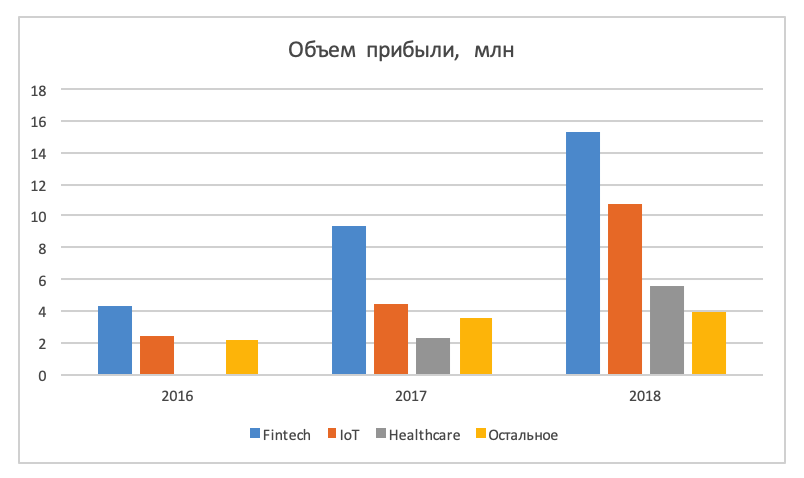
\includegraphics[scale=1]{figures/sampadIncome.png}
	\caption{Прибыль компании Sampad в различных сферах}
	\label{fig:analysis:companyGarlands:sampadIncome}
\end{figure}

Перед началом проекта по управлению адресными светодиодными лентами, было проведено маркетинговое исследование. Данное исследование выявило самую эффективную платформу для разработки приложения~--- мобильные устройства (Рисунок \ref{fig:analysis:companyGarlands:deviceMarket}). Мобильные телефоны имеются практически у каждого человека, так что выбор данной платформы позволяет совершить самый широкий обхват пользователей. Также мобильные устройства отлично подходят для управления различными устройствами в сети, в том числе и адресной светодиодной лентой.

~
\begin{figure}[H]
\centering
	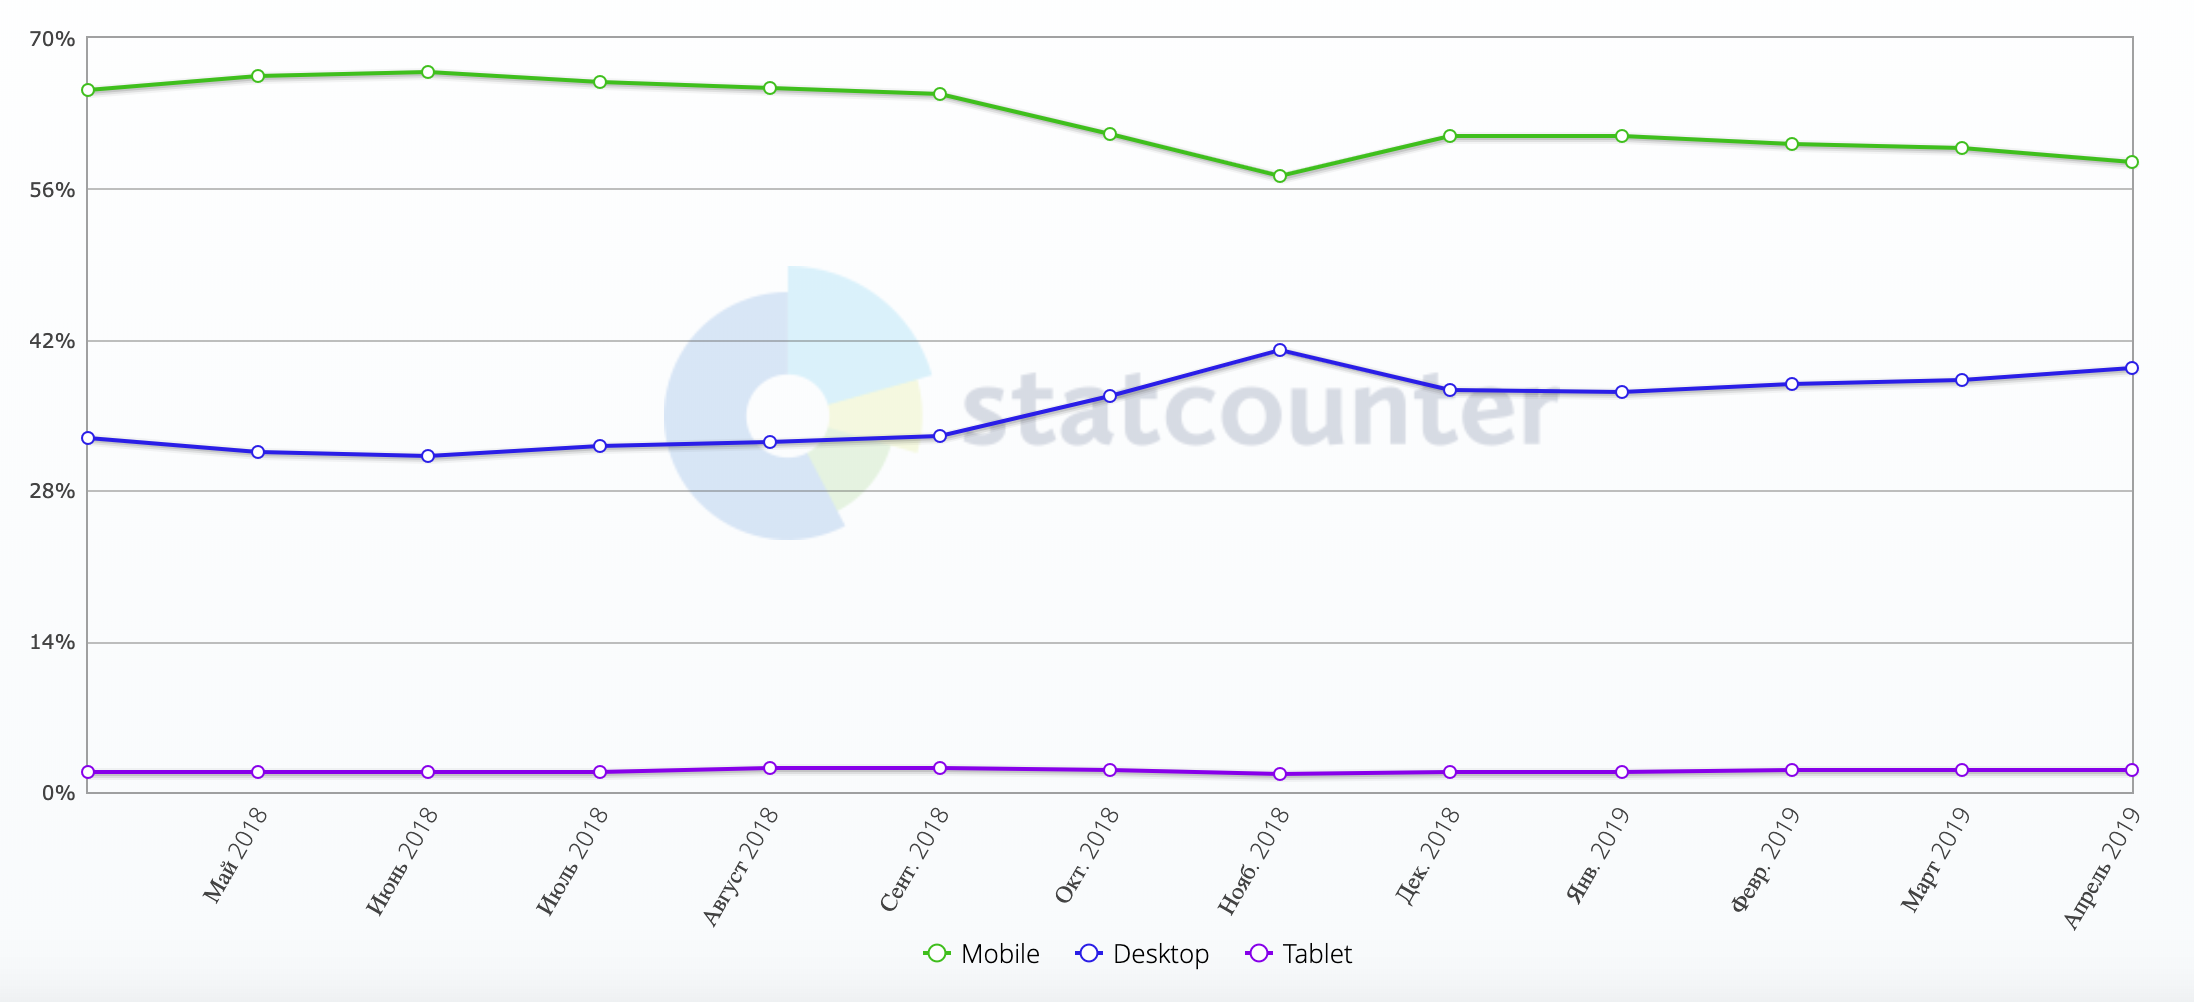
\includegraphics[scale=0.4]{figures/deviceMarket.png}
	\caption{Сравнение количества мобильных устройств, компьютеров и планшетов}
	\label{fig:analysis:companyGarlands:deviceMarket}
\end{figure}

Также были исследованы обе мобильные операционные системы (iOS и Android), и, исходя из полученных данных, было принято решение первоначально сделать приложения для операционной системы Apple iOS (Рисунок \ref{fig:analysis:companyGarlands:digitalMarkets}). Данная операционная система является закрытой и имеет только один, проприетарный магазин приложений. В данных условиях приложение по управлению адресными светодиодными лентами имеет доступ к наиболее полному набору пользователей данной операционной системы.

~
\begin{figure}[H]
\centering
	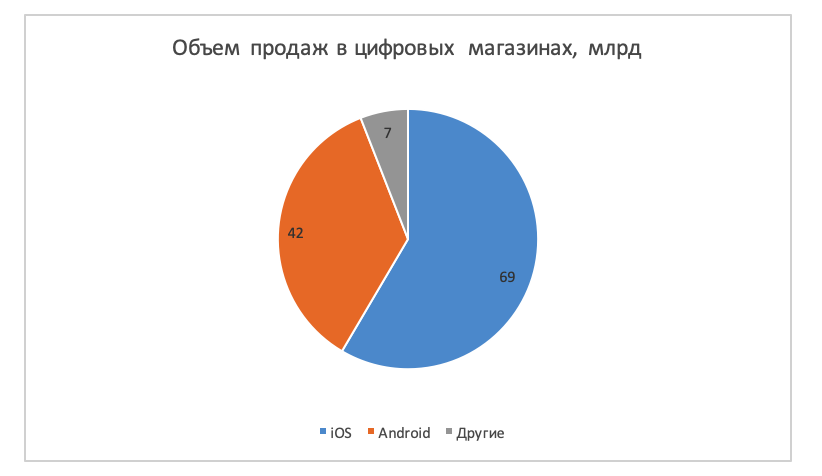
\includegraphics[scale=1]{figures/digitalMarkets.png}
	\caption{Сравнение объема продаж в цифровых магазинах в различных операционных системах}
	\label{fig:analysis:companyGarlands:digitalMarkets}
\end{figure}

По результатам исследования и маркетинговым прогнозам, приложение должно принести большую прибыль компании. Более подробное экономическое обоснование представлено в главе 4.